\documentclass[tc]{unisc}

\usepackage[T1]{fontenc}        % Suporte a acentuação no arquivo de saída
\usepackage[utf8]{inputenc}     % Codificação dos arquivos de entrada em UTF-8
\usepackage[english,brazilian]{babel}

\usepackage{graphicx}           % Para adicionar figuras
\usepackage{float}              % Maior controle de objetos "float" (tabelas, figuras, etc.)

\usepackage{capt-of}
\usepackage{longtable}
\usepackage{tabularx}

\graphicspath{ {images/} }


% ==================================================================================
%
%                         INFORMAÇÕES GERAIS
%
% ==================================================================================

\title{Ambiente de recomendação de índices para bancos de dados MySQL}

\author{Weiland}{Eduardo}
\advisor[Prof. Msc.]{Kroth}{Eduardo}
\reviewer[Prof. Msc.]{Molz}{Kurt Werner}
\reviewer[Prof. Msc.]{Franzen}{Evandro}

\dept{Departamento de Computação}
\course{Curso de Ciência da Computação}
\degree{Bacharel em Ciência da Computação}
\location{Santa Cruz do Sul}{RS}
\date{23}{junho}{2016}

\makeindex

% ==================================================================================
%
%                         CONTEÚDO
%
% ==================================================================================


\begin{document}

\makecapa
\maketitle

% Dedicatória é um elemento opcional.
% Deve ser utilizado o ambiente dedicatoria:

\begin{dedicatoria}
  A todos os usuários do \emph{\LaTeX}!
\end{dedicatoria}

% Agradecimentos é um elemento opcional.
% Deve ser utilizado como um capítulo normal, sem numeração:

\chapter*{Agradecimentos}

Texto de agradecimento.

% Resumo em língua vernácula é um elemento obrigatório.
% Deve ser utilizado o ambiente abstract e o comando \keywords deve ficar no começo:

\begin{abstract}
  \keywords{MySQL, recomendação de índices, modelo físico}
  
  Ferramentas para recomendação de índices são utilizadas para auxiliar na definição dos índices que devem ser criados em um banco de dados relacional, visando obter um melhor desempenho para execução de consultas. Vários bancos de dados já oferecem ferramentas com esse objetivo, como Microsoft SQL Server, Oracle Database, IBM DB2 e PostgreSQL. O presente trabalho apresenta o desenvolvimento de um ambiente para recomendação de índices para bancos de dados MySQL. O ambiente analisa uma carga de trabalho composta de diversas consultas SQL. Essa carga de trabalho é carregada para a ferramenta a partir de um arquivo XML em um formato pré-definido. Cada consulta é interpretada e um conjunto de índices candidatos será gerado. Os índices são, então, criados em um banco de dados configurado pelo usuário do ambiente, que já deve conter todas as tabelas e dados necessários. Os índices candidatos são avaliados através de instruções EXPLAIN, calculando o custo de todas as consultas utilizando cada índice possível. A saída ao final da execução da ferramenta é o conjunto de índices recomendados que oferece o menor custo total para a carga de trabalho.
\end{abstract}

% Resumo em língua estrangeira é um elemento obrigatório:
% Deve ser utilizado o ambiente abstract com duas opções:
%   - Idioma a ser utilizado (no exemplo abaixo, english)
%   - Título do capítulo (deve ser a tradução de "Resumo" para o idioma utilizado)
%
% O comando \keywords também deve ser utilizado com uma opção extra:
%   - Rótulo para as palavras-chave (deve ser a tradução de "Palavras-chave" no idioma utilizado)
%

\begin{abstract}[english][Abstract]
  \keywords[Keywords]{MySQL, index advisor, physical model}

  Index advisor tools are used to assist in the definition of indexes that should be created in a relational database in order to obtain better performance for running queries. Several databases already offer tools for this purpose, such as Microsoft SQL Server, Oracle Database, IBM DB2 and PostgreSQL. This paper proposes the development of an index advisor environment for MySQL databases. The environment analyzes a workload consisting of several SQL queries. This workload is loaded into the tool from an XML file in a predefined format. Each query is interpreted and a set of candidate indexes is generated. The indexes are then created in a database configured by the user, which should already contain all the tables and data required. Candidate indexes are evaluated by EXPLAIN statements, calculating the cost of all queries using every possible index. The output at the of the execution is a  set of recommended indexes that offers the lowest total cost to the workload.
\end{abstract}

\listoffigures
\listoftables
\lstlistoflistings
% Ajuste do tamanho da coluna que contém a descrição da abreviatura.
% Precisa ser reduzido quando uma abreviatura maior for adicionada.
\setlength{\glsdescwidth}{14cm}

% Lista de abreviaturas:
\newacronym{dba}{DBA}{\textit{Database System Administrator}}
\newacronym[longplural={Sistemas de Gerenciamento de Banco de Dados}]{sgbd}{SGBD}{Sistema de Gerenciamento de Banco de Dados}
\newacronym{sql}{SQL}{\textit{Structured Query Language}}
\newacronym{api}{API}{\textit{Application Programming Interface}}
\newacronym{odbc}{ODBC}{\textit{Open Database Connectivity}}
\newacronym{jdbc}{JDBC}{\textit{Java Database Connectivity}}
\newacronym{dml}{DML}{\textit{Data Manipulation Language}}
\newacronym{ddl}{DDL}{\textit{Data Definition Language}}
\newacronym{mdc}{MDC}{\textit{Multidimensional Clustering}}
\newacronym{xml}{XML}{\textit{eXtensible Markup Language}}
\newacronym{json}{JSON}{\textit{JavaScript Object Notation}}

\printglossary     % Esse comando "print" apenas gera a lista de abreviaturas
\printacronyms     % Esse comando exibe a lista gerada no comando anterior

\tableofcontents

\chapter{Introdução}
\label{introducao}

É essencial para quase todos os \emph{softwares} ter um bom desempenho, seja por necessidade dos clientes ou para oferecer uma melhor experiência para os usuários, esse é um fator cada vez mais importante em muitas aplicações, e diretamente relacionado à forma em que os dados são armazenados e acessados. Atualmente, os \glspl{sgbd} relacionais são um dos meios de armazenamento mais utilizados no desenvolvimento de novas aplicações \cite{Heuser:2009}.

A melhoria do desempenho de bancos de dados relacionais consiste em identificar quais são os principais problemas de performance e tentar resolvê-los \cite{Thalheim:2011}. Os problemas mais comuns podem ser configurações de \emph{hardware} do servidor inadequadas, consultas escritas de forma não otimizada, ou a organização física dos dados em disco não corresponder às necessidades da aplicação.

A modelagem física de um banco de dados é o processo que define a organização física dos dados em disco, e compreende a definição de índices, particionamento, agrupamento (\emph{clustering}) e materialização de dados \cite[p. 7]{Lightstone:2007}. A otimização manual dessa modelagem é uma tarefa complexa e que exige muito conhecimento técnico por parte do administrador do banco de dados -- \gls{dba}. Com isso, a necessidade de ferramentas que automatizem esse processo é cada vez mais importante \cite{Alagiannis:2010}.

A otimização do modelo físico é vista pelos autores da área como a estratégia mais eficiente para melhorar o desempenho dos \glspl{sgbd} \cite{Thalheim:2011,Zilio:2004}. Segundo \citet{Petraki:2015}, dentre as possíveis melhorias no esquema físico de um banco de dados, a escolha de índices adequados ainda é a que apresenta os melhores resultados. Algumas das técnicas empregadas para otimização de índices mais conhecidas e aplicadas são \emph{offline}, \emph{online} e adaptativa.

A indexação \emph{offline} foi a primeira estratégia adotada pelos \glspl{sgbd} comerciais. Consiste em uma ferramenta que auxilia o trabalho do \gls{dba}, analisando uma determinada carga de trabalho (\emph{workload}) e sugerindo melhorias. Porém, essa técnica requer o conhecimento prévio da carga de trabalho a qual o servidor deve estar preparado, o que nem sempre é possível, visto a dinamicidade das aplicações modernas.

Por sua vez, a indexação \emph{online} surgiu como uma alternativa para resolver o maior problema da indexação \emph{offline}, sugerindo uma abordagem em que a carga de trabalho do servidor é monitorada continuamente. Conforme a carga de trabalho sofre alterações, novos índices podem ser criados e índices já existentes podem ser atualizados ou excluídos conforme a necessidade. No entanto, tais operações requerem um longo tempo para completar e consomem mais recursos de processamento, tornando-se inviáveis para bancos com um maior volume de dados.

A estratégia de indexação adaptativa aparece como uma opção mais econômica no uso de recursos, enquanto ainda resolve o problema de não ter um conhecimento prévio da carga de trabalho. Essa técnica consiste em realizar pequenas atualizações de forma incremental nos durante a execução de cada consulta. Dessa forma, os índices se mantém sempre atualizados e instantaneamente preparados para a carga de trabalho à qual o servidor é submetido.

Os trabalhos desenvolvidos mais recentemente sugerem, geralmente, uma abordagem \emph{online} ou adaptativa, ou ainda uma nova aproximação, como a abordagem holística proposta por \citet{Petraki:2015}. Poucos trabalhos continuam explorando a técnica de indexação \emph{offline}. No entanto, em aplicações onde a carga de trabalho do banco de dados é razoavelmente constante e previsível, as técnicas de otimização \emph{online} e adaptativa são desnecessárias.

Nessas condições, os sistemas obteriam maiores benefícios tendo um modelo físico definitivo adaptado e otimizado à maioria das condições de operação normal da aplicação. Isso auxiliaria na redução de custos de manutenção do banco de dados ao longo do tempo, além de evitar estressar o sistema continuamente com as verificações de performance do modelo físico realizadas pelas técnicas de otimização mencionadas acima. Dessa forma, uma abordagem \emph{offline} ainda pode ser aplicada em casos específicos.

O objetivo geral desse trabalho é desenvolver um ambiente de código aberto para recomendação de índices para bancos de dados MySQL, visando obter um conjunto de índices equilibrado que oferece um bom desempenho geral para um determinado conjunto de consultas.

Os objetivos específicos do presente trabalho são:

\begin{itemize}
  \item Verificar quais as principais características que influenciam a performance dos bancos de dados relacionais em geral;
  \item Definir um modelo de avaliação de performance do \gls{sgbd} para comparar os resultados obtidos com a solução desenvolvida e as ferramentas já existentes no mercado;
  \item Elaborar a ferramenta de forma que possibilite o desenvolvimento futuro de integração com diferentes \glspl{sgbd};
  \item Validar a solução desenvolvida em um ambiente de uso real.
\end{itemize}

O trabalho é estruturado da seguinte forma: no capítulo \ref{arquitetura-bd} são descritos os principais componentes que formam a arquitetura geral de um banco de dados relacional; o capítulo \ref{estrategias-otimizacao} introduz alguns aspectos importantes relacionados à otimização de um banco de dados; o capítulo \ref{trabalhos-relacionados} apresenta alguns trabalhos relacionados e realiza uma comparação entre esses e o presente trabalho; já no capítulo \ref{solucao-desenvolvida} é apresentada a solução que foi desenvolvida. O trabalho encerra apresentando os resultados e conclusões obtidos e as referências utilizadas.

\chapter{Arquitetura de bancos de dados}
\label{arquitetura-bd}

A arquitetura básica de um banco de dados relacional é composta de um cliente e de um servidor, como pode ser visualizado na figura \ref{fig:client-server}. O cliente possui poucas funcionalidades próprias, sendo utilizado apenas como interface entre o servidor e o usuário. O servidor, por outro lado, é responsável por todo o processamento das consultas. Essa separação entre cliente e servidor favorece a independência de dados, onde o cliente não precisa saber como os dados são fisicamente armazenados, simplificando o desenvolvimento de novas aplicações \cite[p. 30]{Bell:2012}.

A comunicação entre aplicações cliente e servidor geralmente é feita através de uma conexão de rede, mas também pode ser realizada por estruturas internas do sistema operacional (\emph{sockets}, \emph{pipes}, etc.) ou integrando-se o banco de dados à aplicação (\gls{sgbd} embarcado). Qualquer que seja o meio de comunicação utilizado, o cliente envia consultas para o servidor, que a processa e retorna o resultado para o cliente.

\begin{figure}[H]
  \centering
  \caption{Modelo de comunicação cliente/servidor em bancos de dados relacionais.}
  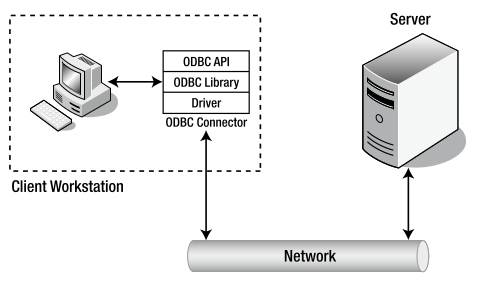
\includegraphics[width=.65\textwidth]{images/client-server-model.png}
  \fonte{\citet[p. 28]{Bell:2012}}
  \label{fig:client-server}
\end{figure}

Nas seções seguintes é descrita a estrutura interna de cada um dos elementos que compõem a arquitetura de um banco de dados relacional. A seção \ref{modelo-relacional} descreve o modelo relacional proposto por E. F. Codd, no qual os \glspl{sgbd} relacionais são baseados. Na seção \ref{aplicacao-cliente} é abordado o funcionamento da aplicação cliente, bem como a forma de apresentação das consultas e dos resultados. A seção \ref{interface-comunicacao} descreve como é feita a comunicação entre as aplicações cliente e servidor, e as estruturas utilizadas para esta finalidade. Por fim, a seção \ref{processamento-consultas} expõe as etapas de processamento das consultas no servidor, incluindo os estágios de análise léxica e sintática, a geração do plano de execução e a efetiva realização da operação requisitada pelo cliente.



\section{Modelo relacional}
\label{modelo-relacional}

O modelo de dados relacional proposto inicialmente por E. F. Codd em 1970 define o conceito de um método de armazenamento de dados que pode ser acessado e manipulado utilizando uma linguagem de consulta \cite[p. 25]{Bell:2012}. Devido à sua simplicidade e bom embasamento teórico e matemático, o modelo tornou-se o mais utilizado para armazenamento de dados estruturados \cite{Lightstone:2007}.

No modelo relacional, os dados são representados como informações (atributos) sobre uma determinada entidade. Um registro ou tupla contém os valores para os atributos de uma entidade. As tabelas são um conjunto de registros que possuem os mesmos atributos, e podem ser relacionadas a outras tabelas utilizando-se restrições (\emph{constraints}).

Não existe uma linguagem de consulta padrão definida pelo modelo relacional. Contudo, muitas aplicações optaram por implementar a \gls{sql}, uma linguagem de consulta que se assemelha com linguagem natural. Atualmente, a \gls{sql} é o padrão do mercado, sendo suportada pelos \glspl{sgbd} mais conhecidos e utilizados \cite[p. 26]{Bell:2012}.



\section{Aplicação cliente}
\label{aplicacao-cliente}

Uma aplicação cliente pode ser qualquer \emph{software} que se comunique com o \gls{sgbd} para manipular os dados de alguma forma. Essa definição inclui tanto aplicações desenvolvidas para serem utilizadas por usuários finais quanto aplicações de gerenciamento e modelagem do banco de dados. Qualquer \emph{software} cliente envia comandos para o servidor utilizando, geralmente, a linguagem \gls{sql}, recebe a resposta e exibe para o usuário.

Os comandos \gls{sql} podem ser divididos em duas categorias principais: \gls{ddl}, utilizada para criação das estruturas de armazenamento dos dados, como tabelas e índices, e a \gls{dml}, responsável pelas operações de manipulação dos dados armazenados, como criação de novos registros, modificação dos dados já existentes e recuperação dos dados salvos.

Cada comando \gls{sql} possui uma sintaxe própria e bem-definida. Todos possuem a especificação de uma ação, por exemplo criar uma tabela (CREATE TABLE) ou atualizar dados (UPDATE). Em seguida são informados demais parâmetros que afetam o tipo de estrutura que será criado ou os dados que serão atingidos.



\section{Interface de comunicação}
\label{interface-comunicacao}

Existem, de maneira geral, duas diferentes formas de comunicação entre uma aplicação cliente e o \gls{sgbd}. Em uma delas, o cliente e o servidor são processos separados, e a comunicação ocorre utilizando alguma interface de rede ou estruturas especiais oferecidas pelo sistema operacional, como \emph{pipes}, \emph{FIFOs} e \emph{sockets}. Esse meio de comunicação é o mais comum e é utilizado na maioria das aplicações modernas. Utilizam o conceito de envio de consultas \gls{sql} para o servidor e o retorno da resposta para o cliente utilizando um protocolo de comunicação padronizado, geralmente o \gls{odbc} ou uma de suas variantes, como o \gls{jdbc}. Estes protocolos definem o formato das mensagens enviados entre cliente e servidor, além de promover uma forma de acesso padrão para diferentes \glspl{sgbd}.

Outra forma de comunicação é o uso de um \gls{sgbd} embarcado. Dessa forma, a aplicação cliente utiliza funções disponibilizadas em uma \gls{api} fornecida pelo banco de dados para acessar diretamente os arquivos de armazenamento dos dados. O exemplo de banco de dados mais conhecido que oferece essa funcionalidade é o SQLite\footnote{SQLite: http://sqlite.org/}, porém outros bancos de dados também oferecem suporte a essa opção \cite[p. 195]{Bell:2012}. Mesmo nessa modalidade, as consultas ainda são escritas em \gls{sql} ou em outra linguagem suportada.



\section{Processamento de consultas}
\label{processamento-consultas}

Em bancos de dados que seguem o modelo cliente/servidor, o processamento das consultas é feito de forma sequencial no servidor e separado em várias etapas. Cada etapa é responsável por realizar alguma operação ou transformação sobre a consulta e gerar uma saída, que será utilizada na próxima etapa. Uma visão geral do processo de execução das consultas é exibido na figura \ref{fig:etapas-execucao-consulta}.

\begin{figure}[ht]
  \centering
  \caption{Etapas do processamento de consultas em um SGBD relacional.}
  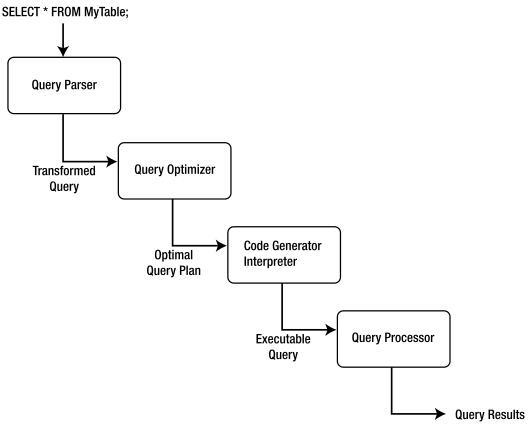
\includegraphics[width=.8\textwidth]{images/etapas-execucao-consulta.png}
  \fonte{\citet[p. 33]{Bell:2012}}
  \label{fig:etapas-execucao-consulta}
\end{figure}

A primeira tarefa executada quando uma nova consulta é recebida pelo servidor é a análise e interpretação do seu significado (\emph{Query Parser}). Considerando uma consulta escrita em \gls{sql}, é necessário identificar os atributos e tabelas que o cliente deseja acessar, e quais as condições definidas para restringir os registros que devem ser retornados. Todas essas informações devem ser extraídas da consulta recebida e convertidas para uma estrutura com a qual o \gls{sgbd} possa trabalhar nas etapas seguintes.

A consulta é convertida para uma estrutura em árvore identificando os componentes da lógica relacional, isto é, quais atributos devem ser retornados (projeção), quais junções entre tabelas devem ser realizadas, quais critérios de seleção devem ser aplicados e, caso indicado na consulta, as funções de agregação e ordenação que devem ser aplicadas. Todas essas informações formam a estrutura gerada pela etapa de análise da consulta.

Após a criação da árvore de consulta, na etapa seguinte (\emph{Query Optimizer}) são identificadas as possíveis abordagens para acesso aos dados e realização da junção entre tabelas. Essa tarefa é executada pelo otimizador, que é responsável por montar um plano de execução otimizado para a consulta a ser efetuada.

Existem quatro principais meios de otimização de consultas que são utilizados em \glspl{sgbd} relacionais \cite{Bell:2012}. 1) A otimização baseada em custo gera vários planos de execução equivalentes e então escolhe o que possui o menor custo, baseado em estatísticas coletadas em consultas anteriores. 2) A otimização heurística implementa algumas boas práticas para execução da consulta, utilizando algumas regras para eliminar os casos que provavelmente apresentariam um desempenho ruim e sugerindo opções que possivelmente apresentem alguma melhoria na performance.

A combinação dos métodos de otimização baseada em custo e heurísticas resulta na (3) otimização paramétrica, visando reduzir a quantidade de planos de execução a serem avaliados, através do uso de funções heurísticas para ignorar os piores planos. Uma quarta alternativa, que ainda não é implementada em \glspl{sgbd} comerciais, é a (4) otimização semântica, que ainda está em pesquisa, cujo objetivo é que o otimizador tenha conhecimento do esquema do banco de dados e das restrições existentes, simplificando partes da consulta automaticamente.

A saída do otimizador é o plano de execução que foi escolhido de acordo com os parâmetros de performance como sendo o mais otimizado. Na etapa seguinte (\emph{Code Generator Interpreter}), o plano é convertido em um algoritmo para acessar as estruturas físicas de armazenamento dos dados, como os índices e as tabelas. A etapa de execução da consulta (\emph{Query Processor}) pode ser implementada utilizando duas estratégias: iterativa e interpretativa.

A estratégia interpretativa consiste em transformar o plano de execução em uma sequência de chamada de funções pré-compiladas. As funções utilizadas são implementadas de forma genérica e executam tarefas básicas do processamento da consulta, não sendo otimizadas para nenhum caso específico. É a mais utilizada em sistemas de bancos de dados relacionais \cite[p. 35]{Bell:2012}.

Na estratégia iterativa, o \gls{sgbd} implementa funções para operações discretas (junção, projeção, etc.). O processamento da consulta consiste na transformação do plano de execução em um programa que utiliza essas funções disponibilizadas pelo banco de dados e subsequente compilação do mesmo em um arquivo binário executável.

Para recuperar as informações solicitadas, o \gls{sgbd} precisa definir como será feito o acesso aos dados no disco. A estrutura mais utilizada nos bancos de dados modernos são arquivos, acessados por meio do sistema de arquivos do sistema operacional. Um motor de armazenamento (\emph{storage engine}) estabelece a estrutura e forma de acesso aos arquivos, tendo como principal objetivo minimizar os custos de operações de entrada e saída (E/S). Com essa finalidade, alguns dos métodos mais empregados são o uso de estruturas que permitam acessar apenas as informações relevantes do disco, um mecanismo de \emph{cache} ou \emph{buffer} para aprimorar o tempo de leitura dos dados, e o uso de índices para auxiliar a obter os registros desejados.

\chapter{Estratégias de otimização}
\label{estrategias-otimizacao}

Nas próximas seções são detalhadas algumas das estruturas e técnicas utilizadas pelos \glspl{dba} quando se deseja obter um melhor desempenho na execução das consultas em bancos de dados relacionais. Na seção \ref{indices} é detalhado o assunto de indexação, mencionando os vários tipos de índices existentes e como são utilizados. A seção \ref{outras-otimizacoes} descreve brevemente outras abordagens existentes para otimização de bancos de dados, como particionamento, visões materializadas e agrupamento de dados.


\section{Índices}
\label{indices}

Um índice é uma estrutura de dados auxiliar utilizada pelo \gls{sgbd} durante a execução de uma consulta para encontrar os dados mais rapidamente \cite[p. 53]{Lightstone:2007}. O uso de índices como forma de localizar dados específicos em um banco de dados é uma das formas mais comuns de otimização e também a que apresenta o melhor resultado quando os índices corretos são selecionados \cite{Petraki:2015}. De forma geral, os índices podem ser classificados em simples ou compostos, primários ou secundários e únicos ou não-únicos.

Os índices simples são formados por apenas um atributo da tabela. Dessa forma, a chave do índice é o valor do atributo indexado, e o índice informa a localização de um ou mais registros da tabela que possuem o mesmo valor da chave para esse atributo. Os índices compostos são criados para múltiplos atributos de uma mesma tabela. A chave do índice, nesse caso, é formada pela concatenação dos valores dos atributos indexados, e indica a localização de registros que possuam os mesmos valores concatenados da chave para os mesmos atributos. Os índices compostos apresentam um desempenho melhor do que o uso de índices simples quando os dados são filtrados por mais de um atributo presente no índice, porém sua utilização é restrita apenas às consultas que se encaixam em alguns critérios \cite[p. 21]{Lightstone:2007}. A ordem dos atributos no índice é importante, uma vez que a chave é formada pela concatenação dos valores, as consultas devem incluir os atributos que estão no começo da chave para utilizar o índice.

Os índices primários definem a organização principal dos dados na tabela. A chave desse tipo de índice, também conhecida como chave primária, deve ser um valor único para cada registro. Esse é um dos índices mais importantes em uma banco de dados, pois a maioria das junções entre tabelas é feita através da chave primária \cite[p. 56--57]{Lightstone:2007}. Cada tabela pode possuir um único índice primário, e todos os outros índices da tabela são chamados de secundários.

Índices únicos são formados por atributos cujos valores não podem ser repetidos em toda a tabela. Todos os índices primários devem ser índices únicos, mas índices secundários também podem ser definidos como tal. Cada entrada em um índice único identifica exclusivamente um registro na tabela, enquanto que em índices não-únicos para cada valor da chave podem existir vários identificadores de linhas na tabela.

Os \glspl{sgbd} relacionais oferecem diferentes estruturas para definição dos índices, sendo as principais e mais utilizadas: \emph{B+tree}, \emph{hash} e \emph{bitmap}. Estas estruturas definem como os dados do índice são organizados em disco e acessados posteriormente na etapa de execução da consulta.

Os índices \emph{B+tree} utilizam uma estrutura de árvore com ponteiros para blocos de dados. O tamanho da árvore varia de acordo com a quantidade de valores distintos existentes para os atributos que compõem o índice. Os nós intermediários da árvore possuem os valores dos atributos ordenados e ponteiros para sub-árvores de busca. Esses valores são utilizados para identificar qual sub-árvore contém a chave pesquisada, reduzindo o espaço de busca e possibilitando encontrar os nós folha de forma eficiente, com poucas operações de entrada/saída de dados.

Os nós folha dos índices \emph{B+tree} possuem as informações realmente importantes: a chave, que são os valores dos atributos que compõem o índice, um identificador de um ou mais registros da tabela que possuem o valor da chave, a partir do qual o \gls{sgbd} pode localizar precisamente a linha indicada, e um ponteiro para o próximo nó folha da árvore, que agiliza buscas por intervalos de valores, acessando diretamente os nós folha sem caminhar pela árvore.

O desempenho desse tipo de índice depende diretamente de sua seletividade, como mostra a figura \ref{fig:btree-index-vs-table-scan}. O tempo necessário para o acesso sequencial à tabela é constante, enquanto que o tempo para leitura dos dados utilizando o índice cresce à medida que mais registros são retornados pela consulta.

\begin{figure}[ht]
  \centering
  \caption{Tempo de acesso ao disco utilizando índice \emph{B+tree} vs. acesso sequencial.}
  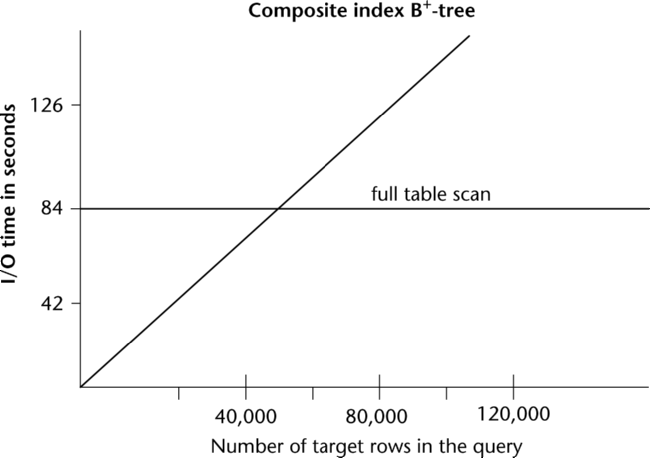
\includegraphics[width=.7\textwidth]{btree-index-vs-table-scan.png}
  \fonte{\citeonline{Lightstone:2007}}
  \label{fig:btree-index-vs-table-scan}
\end{figure}

Os índices do tipo \emph{bitmap} são utilizados para atributos com baixa seletividade, ou seja, com poucos valores diferentes. Cada possível combinação de valores para os atributos do índice possui um vetor de \emph{bits} e cada registro na tabela é representado por um \emph{bit} nesse vetor, sendo que o \emph{bit} é ativado se o registro possui o valor que o respectivo vetor representa. Esse tipo de índice oferece um bom desempenho nas consultas por serem utilizadas operações binárias (E, OU, NÃO) entre os vetores de bits para identificar os registros que possuem uma determinada combinação de valores dos atributos indexados, porém não é facilmente expansível para novos registros e valores de atributos como os índices \emph{B+tree} \cite[p. 27]{Lightstone:2007}.

Índices do tipo \emph{hash} são geralmente utilizados quando os dados de uma tabela não são armazenados em disco de forma ordenada. É utilizada uma função para calcular uma localização em disco a partir do valor da chave, a qual geralmente é criada com atributos que possuem valores únicos. A localização retornada pela função de \emph{hash} identifica o endereço de um bloco inicial, e é utilizado durante as operações de atualização e consulta de dados. Este tipo de índice é recomendado para consultas que acessam um único registro da tabela buscando pelo valor da chave. Entretanto, os índices do tipo \emph{B+tree} oferecem um desempenho equivalente, e, portanto, os índices \emph{hash} são suportados em poucos \glspl{sgbd} \cite[p. 56]{Lightstone:2007}.





\section{Outras otimizações}
\label{outras-otimizacoes}

Além do uso de índices, os \glspl{sgbd} relacionais também oferecem outras estruturas que podem ser utilizadas na definição do modelo físico do banco de dados com o objetivo de reduzir o tempo necessário para acessar os dados. Algumas dessas funcionalidades são o particionamento, as visões materializadas e o agrupamento multidimensional, entre outras menos comuns.

O \textbf{particionamento} é uma técnica de otimização que consiste em dividir grandes volumes de dados em tabelas menores. Existem dois principais métodos para implementar o particionamento: horizontal e vertical. No particionamento horizontal, a estrutura da tabela permanece inalterada, mas o registros são armazenados em arquivos de dados separados. Essa divisão dos dados é feita a partir de algum critério definido previamente pelo \gls{dba}. Nesse tipo de particionamento, os dados são manipulados pelo \gls{sgbd} como se estivessem em tabelas diferentes, com um número menor de registros por tabela, mas para a aplicação que acessa o banco de dados eles continuam sendo apresentados como uma tabela única.

Outra forma de particionamento é o vertical, onde alguns atributos menos utilizados de uma tabela são movidos para outra e apenas uma relação entre os registros é mantida. Assim, o tamanho de cada registro da tabela principal é reduzido, permitindo que o \gls{sgbd} possa carregar mais registros para a memória simultaneamente.

As visões são uma técnica utilizada em bancos de dados para armazenar a definição de uma consulta e permitir que os dados dessa visão sejam acessados posteriormente sem a necessidade de saber como a consulta original foi escrita. As \textbf{visões materializadas} incrementam essa funcionalidade, armazenando o resultado da execução da consulta que forma a visão para que este seja utilizado em consultas subsequentes. Portanto, essa estratégia é útil quando uma determinada visão é acessada frequentemente e não é necessário que o resultado da consulta seja atualizado em todos os acessos.

O agrupamento (\emph{clustering}) simples permite organizar os dados de uma tabela, armazenando os registros que possuem valores de atributos iguais no mesmo bloco em disco. A técnica de \textbf{agrupamento multidimensional} -- \gls{mdc} -- estende o agrupamento simples, permitindo que dentro de um bloco os dados sejam novamente agrupados pelo do valor de outro atributo. Dessa forma, ao executar uma consulta que filtra por um ou mais atributos que fazer parte do agrupamento definido para a tabela, o \gls{sgbd} pode acessar diretamente o bloco no disco que contém as informações desejadas.

\chapter{Trabalhos relacionados}
\label{trabalhos-relacionados}

Este capítulo apresenta alguns dos trabalhos relacionados ao tema estudado referente ao desenvolvimento de uma ferramenta para sugestão de melhorias de performance em um banco de dados.

O trabalho de \textbf{\citeonline{Chaudhuri:1997}} apresentou a proposta de simular a existência de índices em um banco de dados e utilizar o otimizador do \gls{sgbd} para estimar o custo de execução das consultas. Esse mecanismo para simulação de índices no banco de dados foi chamado de \emph{what-if} (e-se), e desde então foi utilizado em diversos outros trabalhos. Ainda, como constatado por \citeonline{Lightstone:2007}, a proposta de \citeauthoronline{Chaudhuri:1997} pode ser interpretada como o uso do otimizador do banco de dados no lugar de uma função de avaliação, utilizado em técnicas de busca em Inteligência Artificial.

No trabalho de \textbf{\citet{Alagiannis:2010}} foi desenvolvida uma ferramenta capaz de recomendar a criação de índices e particionamento de tabelas para bancos de dados PostgreSQL. A solução apresenta uma versão modificada do otimizador de consultas do PostgreSQL, adicionando um componente \emph{what-if} para simular a presença de índices e partições, além de outras ferramentas e módulos que executam isoladamente, como mostra a figura \ref{fig:arquitetura-sistema-alagiannis}.

\begin{figure}[ht]
  \centering
  \caption{Arquitetura do sistema desenvolvido no trabalho de \citeauthoronline{Alagiannis:2010}}
  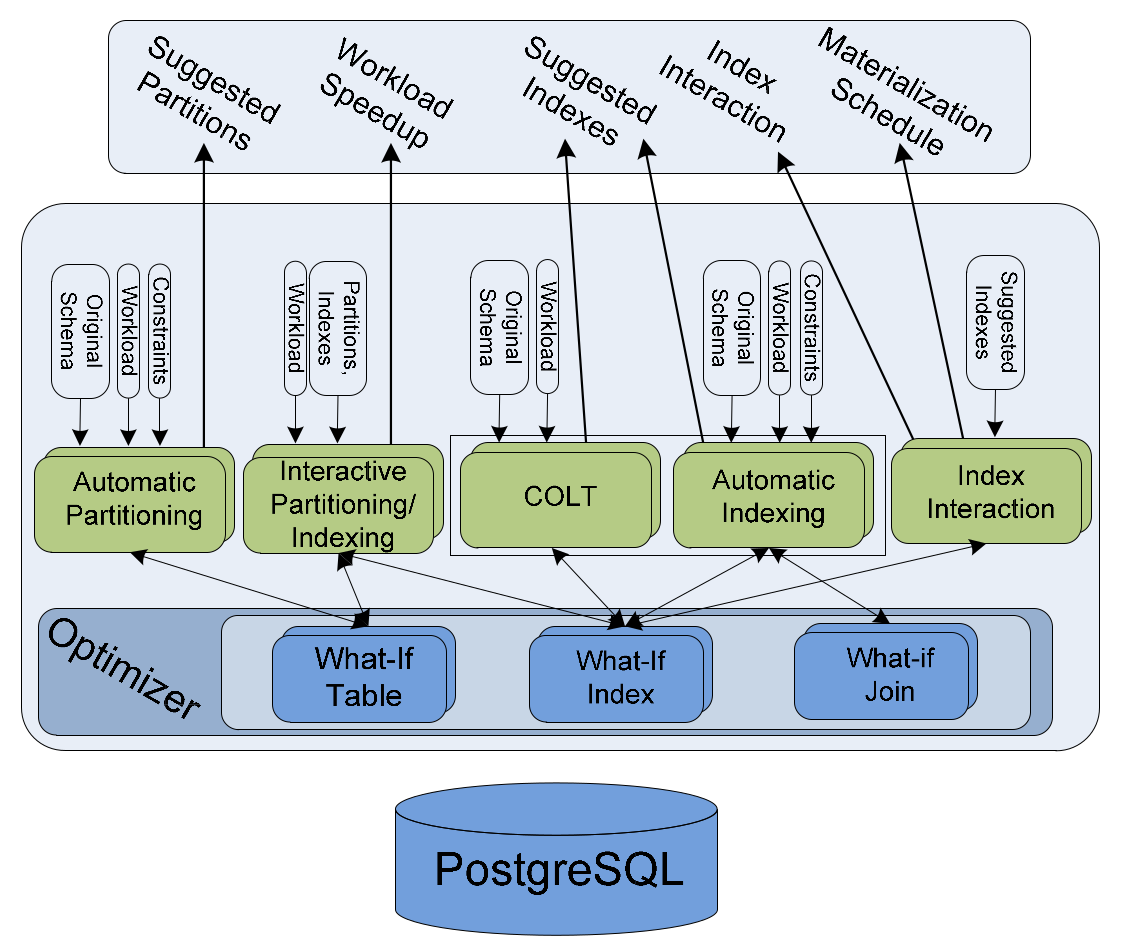
\includegraphics[width=.75\textwidth]{arquitetura-sistema-alagiannis.png}
  \fonte{\citet{Alagiannis:2010}}
  \label{fig:arquitetura-sistema-alagiannis}
\end{figure}

Para realizar recomendações de índices, a ferramenta possibilita duas alternativas: 1) sugestão automática de índices, utilizando uma abordagem \emph{offline}. A ferramenta utiliza o componente CoPhy \cite{Dash:2011} para sugerir os índices candidatos e avalia o custo das consultas utilizando o modelo INUM \cite{Papadomanolakis:2007}. A outra opção para recomendação de índices é a 2) otimização contínua, que utiliza uma abordagem \emph{online} para analisar a carga de trabalho e sugerir modificações nos índices para melhorar a performance. Esta opção é desenvolvida utilizado o \emph{framework} COLT \cite{Schnaitter:2006}, porém as alterações no banco de dados não são realizadas automaticamente, apenas é retornado um novo conjunto de índices recomendados.

O trabalho de \textbf{\citet{Agrawal:2004}} descreve a ferramenta de otimização de banco de dados integrada com o Microsoft SQL Server, o \emph{Database Tuning Advisor} (DTA), apresentada na figura \ref{fig:tela-recomendacoes-sqlserver}. As características que são suportadas por esta ferramenta para análise e recomendação de melhorias são índices, particionamento horizontal e materialização de dados.

\begin{figure}[H]
  \centering
  \caption{Interface da ferramenta \emph{Microsoft SQL Server DTA}.}
  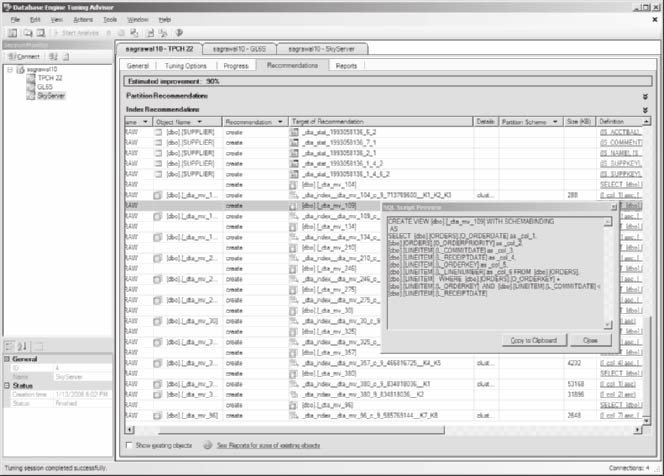
\includegraphics[width=\textwidth]{tela-recomendacoes-sqlserver.png}
  \fonte{\citet{Lightstone:2007}}
  \label{fig:tela-recomendacoes-sqlserver}
\end{figure}

Para realizar a análise e sugestão de índices, a ferramenta utiliza um componente \emph{what-if} nativo do SQL Server, desenvolvido no trabalho de \citet{Chaudhuri:1998}. A ferramenta utiliza uma interface com o otimizador de consultas do \gls{sgbd} para calcular a estimativa de custo das consultas utilizando os índices sugeridos. Os resultados dos experimentos apresentados por \citet{Agrawal:2004} mostram que as sugestões do DTA são superiores às otimizações realizadas manualmente em diferentes cenários, considerando o custo total da carga de trabalho analisada como parâmetro de comparação.

No trabalho de \textbf{\citet{Zilio:2004}} é apresentada a ferramenta \emph{DB2 Design Advisor} (figura \ref{fig:tela-recomendacoes-db2}), desenvolvida para o DB2 Universal Database (DB2 UDB), que oferece a sugestão de um modelo físico composto de índices, partições, visões materializadas e agrupamento multidimensional. O trabalho avalia duas abordagens para resolver o problema: 1) a iterativa, onde cada funcionalidade é sugerida isoladamente, porém pode ocasionar a sugestão de estruturas desnecessárias, e 2) a integrada, onde são avaliadas todas as combinações de funcionalidades e a dependência entre elas para realizar as sugestões.

\begin{figure}[H]
  \centering
  \caption{Interface da ferramenta \emph{DB2 Design Advisor}.}
  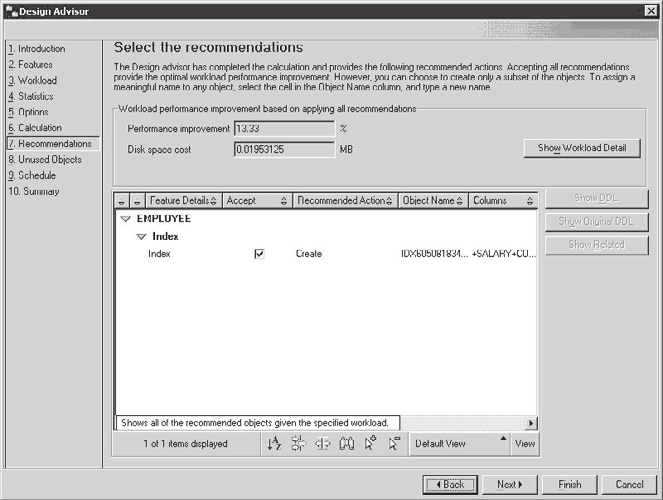
\includegraphics[width=\textwidth]{tela-recomendacoes-db2.png}
  \fonte{\citet{Lightstone:2007}}
  \label{fig:tela-recomendacoes-db2}
\end{figure}

A abordagem escolhida por \citeauthoronline{Zilio:2004} para implementar em seu trabalho foi uma abordagem híbrida, reduzindo o espaço de busca por soluções ao procurar por estruturas que dependem de outras após ter estas definidas. Para calcular a estimativa de custo das consultas foi utilizado um componente \emph{what-if} integrado ao otimizador do DB2. Ao final da execução, a ferramenta exibe uma lista de índices sugeridos e a opção para criá-los no banco de dados. Os resultados obtidos com a ferramenta representaram uma redução do tempo de execução de consultas entre 77\% e 93\% para diferentes casos. A figura \ref{fig:resultados-zilio} apresenta os resultados obtidos utilizando um banco de dados derivado de um \emph{benchmark} TPC-H\footnote{TPC Benchmark H: \url{http://www.tpc.org/tpch/default.asp}}, que consiste em um grande volume de dados e um conjunto de consultas complexas, criado especificamente para avaliações de desempenho.

\begin{figure}[H]
  \centering
  \caption{Resultados obtidos por \citeauthoronline{Zilio:2004} utilizando um banco de dados TPC-H.}
  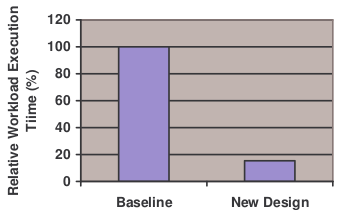
\includegraphics[width=.5\textwidth]{resultados-zilio.png}
  \fonte{\citet{Zilio:2004}}
  \label{fig:resultados-zilio}
\end{figure}

O \textbf{Percona Toolkit}\footnote{Percona Toolkit: \url{http://www.percona.com/software/mysql-tools/percona-toolkit}} é um conjunto de ferramentas para auxiliar na manutenção e administração de bancos de dados MySQL. Algumas das ferramentas relacionadas a performance são: identificação de índices duplicados e não utilizados, monitoramento de performance das operações de entrada/saída, análise de consultas lentas, verificação de configurações do \gls{sgbd}, entre várias outras ferramentas para controle de replicação e \emph{backup} \cite{PerconaToolkit:2015}.

\section{Comparativo entre trabalhos relacionados}

A tabela \ref{tab:trabalhos-relacionados} apresenta um quadro comparativo entre os trabalhos relacionados estudados, demonstrando qual o \gls{sgbd} suportado, o objetivo do trabalho, a abordagem utilizada na ferramenta e qual o modelo para avaliação do custo das consultas que foi aplicado.

\begin{table}[H]
  \centering
  \caption{Comparativo de trabalhos relacionados}
  \begin{tabular}{|p{2.1cm}|l|p{4.1cm}|p{2.1cm}|p{3.1cm}|} \hline
    \textbf{Trabalho}
        & \textbf{SGBD}
        & \textbf{Objetivo}
        & \textbf{Abordagem}
        & \textbf{Avaliação de custo}
        \\ \hline

    \citet{Alagiannis:2010}
        & PostgreSQL
        & Sugestão de índices e particionamento
        & \emph{Offline} e \emph{online}
        & Uso de componente \emph{what-if}, acessando otimizador do \gls{sgbd} para avaliar custo da consulta com \emph{cache} dos resultados
        \\ \hline
    \citet{Agrawal:2004}
        & SQL Server
        & Sugestão de índices, particionamento e materialização de dados
        & \emph{Offline}
        & Uso de componente \emph{what-if}, acessando otimizador do \gls{sgbd} para avaliar custo da consulta
        \\ \hline
    \citet{Zilio:2004}
        & DB2
        & Sugestão de índices, particionamento, materialização de dados e agrupamento multidimensional
        & \emph{Offline}
        & Uso de componente \emph{what-if}, acessando otimizador do \gls{sgbd} para avaliar custo da consulta
        \\ \hline
    Percona Toolkit
        & MySQL
        & Análise de configurações, identificação de índices duplicados e não utilizados
        & Não se aplica
        & Não se aplica
        \\ \hline
  \end{tabular}
  \label{tab:trabalhos-relacionados}
  \fonte{Elaborado pelo autor.}
\end{table}

\chapter{Solução desenvolvida -- MIST (\textit{MySQL Index Suggestion Tool})}
\label{solucao-desenvolvida}

A ferramenta MIST (\textit{MySQL Index Suggestion Tool}, Ferramenta de Sugestão de Índices para MySQL) que foi desenvolvida neste trabalho realiza a análise da estrutura de um banco de dados e de um lista de consultas elaboradas para serem executadas nesse mesmo banco, produzindo um conjunto de índices recomendados que podem ser utilizados para otimizar a performance geral do banco de dados.


\section{Modificação da solução proposta}
\label{modificacao-solucao}

A proposta de solução original deste trabalho estabeleceu que seriam realizadas modificações no código-fonte do \gls{sgbd} MySQL a fim de permitir a simulação de índices sem a necessidade de criar sua estrutura completa no banco de dados. Esta decisão em fase de projeto, leia-se TC I, foi dada com base em soluções semelhantes já desenvolvidas para outros \glspl{sgbd} do mercado (SQL Server, Oracle, DB2, entre outros). A partir desta simulação, pretendia-se obter as performances de processamento com os índices sugeridos pelos algoritmos implementados, utilizando os resultados destes testes para gerar a recomendação final da ferramenta.

Depois de uma longa dedicação para conhecer o código-fonte do MySQL, principalmente no que tange à seleção de índices para execução de consultas e seus cálculos de performance, não foi obtido êxito nesta tarefa. Neste período, observou-se que os trabalhos relacionados são frutos de longas pesquisas, fato que não havia sido estimado. Desta forma, resolveu-se modificar o projeto de solução deste trabalho, como descrito na sequência deste capítulo.

As seções a seguir detalham as etapas de desenvolvimento e execução da ferramenta. Na seção \ref{arquitetura-interna} é apresentada de forma sucinta a arquitetura interna do ambiente desenvolvido; na seção \ref{entrada-de-dados} é descrita a forma em que os dados de entrada devem ser apresentados à ferramenta para análise; em \ref{geracao-indices-candidatos} é apresentado o algoritmo que foi implementado para gerar um conjunto de possíveis índices para as consultas examinadas; a seção \ref{verificacao-custo-indices-candidatos} descreve o método que foi utilizado para estimar o custo das consultas com os índices candidatos gerados na etapa anterior; a seção \ref{geracao-solucao-final} apresenta o procedimento realizado para se obter a solução final com a escolha dos índices que apresentam o menor custo total para o banco de dados.


\section{Arquitetura interna}
\label{arquitetura-interna}

O MIST foi desenvolvido para ser utilizado por um administrador do banco de dados que se deseja analisar. O \gls{dba} deve coletar as consultas SQL executadas pela aplicação, o modelo físico do banco de dados e as estatísticas necessárias sobre os dados, convertendo estas informações para arquivos XML utilizados como entrada de dados para a ferramenta, como ilustrado na figura \ref{fig:integracao-solucao}. Como resultado, o ambiente irá apresentar um conjunto de índices recomendados, os quais devem ser avaliados e implementados a critério do \gls{dba}.

\begin{figure}[H]
  \centering
  \caption{Utilização do ambiente desenvolvido.}
  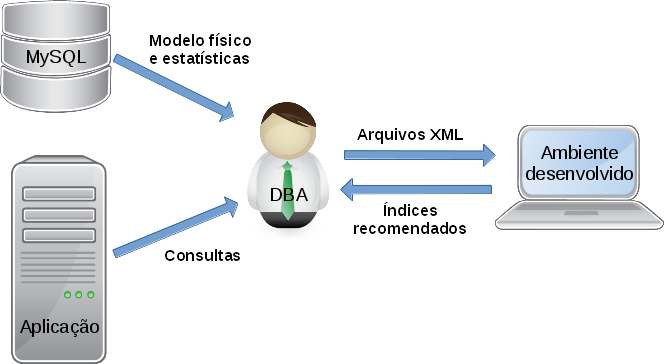
\includegraphics[width=.9\textwidth]{integracao-solucao-tc2.png}
  \fonte{Elaborado pelo autor.}
  \label{fig:integracao-solucao}
\end{figure}

O uso da ferramenta é formado por uma série de operações executadas sequencialmente, conforme apresentado na figura \ref{fig:arquitetura-ambiente}. Na primeira etapa, identificada na figura como (a), é feita a entrada da estrutura das tabelas e as estatísticas dos dados através de um arquivo no formato MSDF (apresentado na seção \ref{formato-msdf}).

\begin{figure}[!ht]
  \centering
  \caption{Arquitetura interna do ambiente desenvolvido.}
  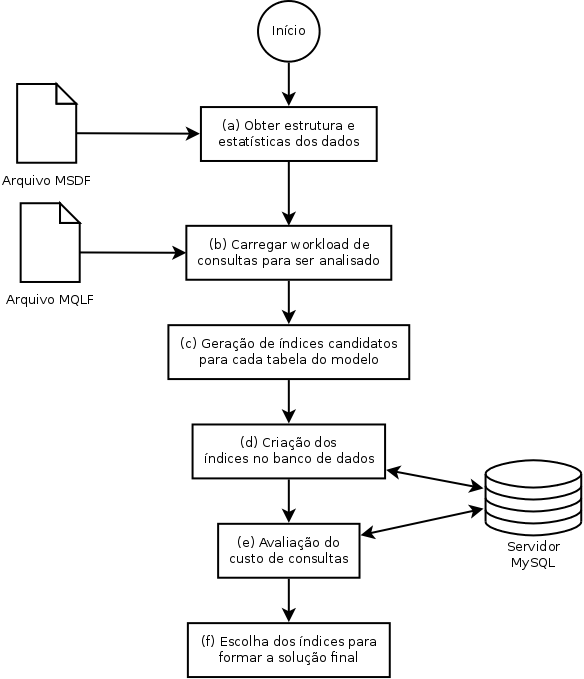
\includegraphics[width=.9\textwidth]{arquitetura-ambiente-tc2.png}
  \fonte{Elaborado pelo autor.}
  \label{fig:arquitetura-ambiente}
\end{figure}

Na etapa (b), o \textit{workload} que deve ser analisado é informado através de um arquivo no formato MQLF, descrito na seção \ref{formato-mqlf}. Em seguida, na fase (c) são gerados os índices candidatos para cada consulta analisada, baseado em boas práticas e recomendações do MySQL. Esta etapa é detalhada na seção \ref{geracao-indices-candidatos}. Posteriormente, em (d) os índices gerados são criados em um banco de dados e o custo das consultas com cada índice é verificado em (e) através de chamadas EXPLAIN para o otimizador do MySQL. Os detalhes destas duas etapas são apresentados na seção \ref{verificacao-custo-indices-candidatos}.

A última etapa (f) da ferramenta consiste em formar o conjunto de índices candidatos que será promovido como recomendação final. Este processo é descrito na seção \ref{geracao-solucao-final}.
\section{Entrada de dados}
\label{entrada-de-dados}

Os dados que são utilizados como entrada para a ferramenta desenvolvida são a estrutura das tabelas, juntamente com algumas estatísticas sobre os dados, e um conjunto de consultas que são executadas por alguma aplicação sobre essas tabelas, igualmente acompanhadas de algumas estatísticas disponíveis.

Para que essas informações sejam apresentadas à ferramenta, foram desenvolvidos dois formatos de arquivos baseados no padrão \gls{xml}. O primeiro deles é o MSDF (\textit{MIST Schema Definition File}, Arquivo de Definição do Modelo do Banco de Dados do MIST), utilizado para descrever a estrutura das tabelas e índices existentes no banco de dados. O outro formato de arquivo é o MQLF (\textit{MIST Query Log File}, Arquivo de Histórico de Consultas do MIST), que descreve um conjunto de consultas para ser analisado.

\subsection{O formato do Arquivo de Definição do Modelo do Banco de Dados (MSDF)}
\label{formato-msdf}

O formato de arquivo MSDF possui uma estrutura como a apresentada no Código \ref{exemplo-formato-msdf}. O elemento raiz da estrutura possui o nome \texttt{schema} e um atributo \texttt{version} que identifica a versão do formato do arquivo. A versão desenvolvida neste trabalho é a \texttt{1.0}, e futuras modificações no formato do arquivo devem incrementar esse valor, de forma que o \textit{software} possa manter compatibilidade com diferentes versões do arquivo.

\begin{lstlisting}[label=exemplo-formato-msdf, caption={Exemplo de arquivo no formato MSDF.}]
<?xml version="1.0" encoding="utf-8" ?>
<schema version="1.0">
    <table name="nome_da_tabela" row-count="50000">
        <column name="id"
                type="integer"
                nullable="false"
                distinct-values="50000"
                null-values="0"/>

        <column name="coluna_int"
                type="integer"
                nullable="true"
                distinct-values="25"
                null-values="3584"/>

        <column name="coluna_texto"
                type="text"
                length="60"
                nullable="true"
                distinct-values="32054"
                null-values="264"/>

        <primary-key>
            <column name="id"/>
        </primary-key>
        <foreign-key table="outra_tabela">
            <column name="coluna_int" referenced="id"/>
        </foreign-key>
    </table>
</schema>
\end{lstlisting}

Os elementos filhos do \texttt{schema} possuem o nome \texttt{table}, representando a estrutura de uma tabela existente do banco de dados. Os atributos deste elemento são \texttt{name}, cujo valor deve ser o nome da tabela, e \texttt{row-count}, que deve informar a quantidade total de registros existentes na tabela. Este e outros valores são utilizados no cálculo de algumas estatísticas sobre os dados no momento da geração de índices candidatos.

Cada coluna de uma tabela é representada no arquivo através de uma \textit{tag} \texttt{column} vazia (contendo apenas atributos) dentro da respectiva \textit{tag} \texttt{table}. O atributo \texttt{name} representa o nome da coluna; o atributo \texttt{type} indica qual é o tipo de dados armazenado na coluna, e deve ser um dos seguintes valores suportados: \texttt{varchar}, \texttt{char}, \texttt{text}, \texttt{tinyint}, \texttt{smallint}, \texttt{integer}, \texttt{mediumint}, \texttt{bigint}, \texttt{boolean}, \texttt{decimal}, \texttt{date}, \texttt{time}, \texttt{datetime}, \texttt{float}, \texttt{double} e \texttt{blob}. O atributo \texttt{nullable} deve conter um valor lógico \texttt{true} ou \texttt{false} indicando se a coluna aceita valores \texttt{NULL} ou não. O atributo \texttt{distinct-values} deve apresentar a quantidade de valores diferentes existentes nessa coluna entre todos os registros da tabela, desconsiderando os valores \texttt{NULL}. Estes devem ser contabilizados no atributo \texttt{null-values}, informando quantos registros possuem o valor \texttt{NULL} para essa coluna. Por fim, os atributos opcionais \texttt{length} e \texttt{precision} são utilizados apenas quando o tipo da coluna requerer essas informações.

Logo após a definição das colunas da tabela devem ser incluídas as definições de chave primária e chaves estrangeiras, quando estas existirem na tabela. Para a chave primária utiliza-se o elemento \texttt{primary-key}, sendo que cada coluna presente na chave primária é indicada através da inclusão de um elemento filho com a \textit{tag} \texttt{column} contendo o atributo \texttt{name}. As chaves estrangeiras são definidas pela inclusão de elementos \texttt{foreign-key}, sendo um para cada chave estrangeira presente na tabela. A \textit{tag} \texttt{foreign-key} possui o atributo \texttt{table} que deve indicar o nome da tabela referenciada. As colunas da chave são indicadas por elementos \texttt{column} filhos, contendo os atributos \texttt{name}, com o nome da coluna na tabela atual, e \texttt{referenced}, com o nome da coluna na tabela referenciada.

\subsection{O formato do Arquivo de Histórico de Consultas (MQLF)}
\label{formato-mqlf}

O arquivo de histórico de consultas (MQLF) apresenta um formato semelhante ao de definição do modelo do banco de dados (MSDF), conforme exemplificado no Código \ref{exemplo-formato-mqlf}. O elemento raiz da estrutura do XML é \texttt{queries}, que possui o atributo \texttt{version} com valor \texttt{1.0}.

\begin{lstlisting}[label=exemplo-formato-mqlf, caption={Exemplo de arquivo no formato MQLF.}]
<?xml version="1.0" encoding="utf-8" ?>
<queries version="1.0">
    <query id="1" count="42">
        <sql>
            SELECT
                t.id,
                t.coluna_texto,
                ot.coluna_int,
                ot.data_compra,
                ot.status,
                SUM(ot.valor)
            FROM
                nome_da_tabela t
            INNER JOIN
                outra_tabela ot
                    ON ot.coluna_int = t.id
            WHERE
                ot.data_compra BETWEEN '2016-01-01' AND '2016-01-31'
                AND ot.status IN ('p', 'a', 'c')
                AND t.coluna_texto LIKE '%pesquisa%'
            GROUP BY
                t.id
            ORDER BY
                t.coluna_texto ASC,
                ot.data_compra DESC
        </sql>
        <from>
            <table>nome_da_tabela</table>
        </from>
        <joins>
            <join type="inner" table="outra_tabela">
                <condition field="coluna_int"
                           type="match"/>
            </join>
        </joins>
        <where>
            <condition table="outra_tabela"
                       field="data_compra"
                       type="range"/>

            <condition table="outra_tabela"
                       field="status"
                       type="list"/>

            <condition table="nome_da_tabela"
                       field="coluna_texto"
                       type="like"/>
        </where>
        <groupby>
            <field table="nome_da_tabela"
                   field="id"/>
        </groupby>
        <orderby>
            <field table="nome_da_tabela"
                   field="coluna_texto"
                   dir="asc"/>

            <field table="outra_tabela"
                   field="data_compra"
                   dir="desc"/>
        </orderby>
    </query>
</queries>
\end{lstlisting}

Os elementos filhos do nodo raiz são identificados pela \textit{tag} \texttt{query}, cada um representando uma consulta distinta executada pelo sistema analisado. Uma consulta é considerada distinta, no contexto deste trabalho, quando não houver outra consulta que apresente, simultaneamente, as mesmas tabelas na cláusula FROM, as mesmas tabelas e condições de junção nas cláusulas JOIN, os mesmos operadores de comparação para os mesmos campos na cláusula WHERE, e os mesmos campos para agrupamento e para ordenação.

O elemento \texttt{query} apresenta ainda os atributos \texttt{id}, que deve ser um número inteiro para identificar exclusivamente cada consulta dentro do mesmo arquivo, e \texttt{count}, que deve ser um número inteiro positivo indicando o número de vezes que essa determinada consulta foi executada dentro de um período observado. O valor deste atributo não necessariamente deve ser exato, mas para obter os melhores resultados a proporção de distribuição do número de execução entre todas as consultas analisadas deve ser mantida próxima ao real.

Os nodos filhos de \texttt{query} são utilizados para descrever a consulta. O primeiro é o \texttt{sql}, que deve conter o texto da consulta original, com todos os valores dos parâmetros necessários para a sua execução no banco de dados. O elemento \texttt{from} deve conter um ou mais elementos \texttt{table} com o nome das tabelas encontradas na cláusula FROM da consulta.

Caso a consulta realize JOINs com uma ou mais tabelas, deve ser incluído o elemento \texttt{joins} para descrevê-los. Este elemento possui nodos filhos com a \textit{tag} \texttt{join}, com um atributo \texttt{type} indicando o tipo de junção realizada (\texttt{inner}, \texttt{left} ou \texttt{right}) e o atributo \texttt{table} com o nome da tabela com a qual é realizado o JOIN. Os nodos filhos desse elemento refletem as condições para a junção, representadas com a \textit{tag} \texttt{condition} e os atributos \texttt{field} com o nome do campo e \texttt{type} com o tipo de comparação utilizado: \texttt{const}, \texttt{match}, \texttt{range}, \texttt{list} ou \texttt{like}.

A \textit{tag} \texttt{where} lista todas as condições de filtro utilizadas no WHERE da consulta SQL. Consiste em vários elementos \texttt{condition} com os atributos \texttt{table} e \texttt{field} identificando, respectivamente, o nome da tabela e o nome do campo que é utilizado na condição, e o atributo \texttt{type} com o tipo do operador de comparação utilizado: \texttt{const}, \texttt{match}, \texttt{range}, \texttt{list} ou \texttt{like}.

Os últimos elementos necessários para descrever a consulta são o \texttt{groupby} e \texttt{orderby}, utilizados apenas no caso de a consulta incluir estes operadores. A \textit{tag} \texttt{groupby} lista os campos utilizados para agrupamento na consulta, utilizando elementos \texttt{field} com os atributos \texttt{table} e \texttt{field} identificando, respectivamente, o nome da tabela e o nome do campo. O elementos \texttt{orderby} lista as regras de ordenação utilizadas na consulta, utilizando \textit{tags} \texttt{field} com os atributos \texttt{table} e \texttt{field} identificando a tabela e coluna ordenada e o atributo \texttt{dir} indicando a direção da ordenação (\texttt{asc} ou \texttt{desc}).

\section{Geração de índices candidatos}
\label{geracao-indices-candidatos}

A geração de índices candidatos envolve analisar as consultas que foram informadas no arquivo de entrada da ferramenta, identificando quais são os campos das tabelas que são incluídos mais frequentemente em condições de filtro, como WHERE e JOIN, bem como em outras cláusulas da consulta que afetam a forma como os dados são recuperados do banco de dados, como GROUP BY e ORDER BY.

O processo de geração dos índices candidatos deve ser otimizado de forma a não sugerir índices que ofereçam ganhos pouco significativos, visando reduzir o tempo de processamento da etapa seguinte - a estimativa de custo das consultas. Com esse objetivo, o MIST foi desenvolvido considerando as recomendações de melhores práticas na criação de índices especificamente para o banco de dados MySQL \cite{MySQL57Ref:Indexes}. Essas recomendações são utilizadas no momento de combinação de colunas para formação dos índices, influenciando na ordem em que as colunas são indexadas, como apresentado na figura \ref{fig:geracao-candidatos}.

\begin{figure}[!ht]
  \centering
  \caption{Processo de geração de índices candidatos.}
  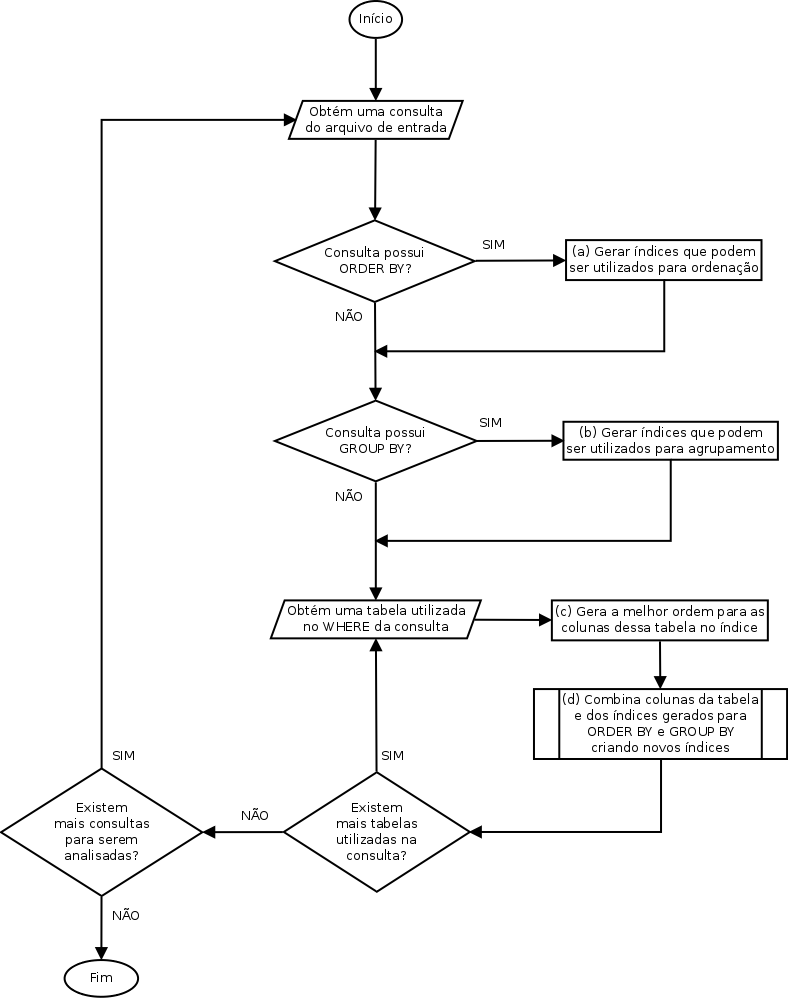
\includegraphics[width=\textwidth]{geracao-candidatos.png}
  \fonte{Elaborado pelo autor.}
  \label{fig:geracao-candidatos}
\end{figure}

Podem ser identificadas nesta figura quatro etapas intermediárias essenciais para a geração dos índices candidatos de forma otimizada, que são executadas para todas as consultas do \textit{workload} analisado. Em (a) são identificadas as colunas incluídas na cláusula ORDER BY da consulta, limitando-se a colunas de uma mesma tabela. Em (b) um processo semelhante é realizado para as colunas da cláusula GROUP BY. A saída dessas duas etapas são os índices mais específicos que podem ser utilizados para ordenação e agrupamento dessa consulta, e são armazenados temporariamente para inclusão em uma etapa posterior.

Após as etapas (a) e (b) serem concluídas, as etapas (c) e (d) são executadas repetidamente para cada tabela diferente incluída na consulta que está sendo analisada. A etapa (c) aplica algumas recomendações e boas práticas para a construção de índices, conforme descrito por \citeonline{Lightstone:2007}. Dessa forma, a implementação do MIST considera uma sequência adequada para escolher as colunas que formarão os índices sugeridos, conforme enumerado a seguir:

\begin{enumerate}
    \item colunas que são utilizadas em comparação de igualdade com valores constantes (parâmetros de comparação informados no SQL) no WHERE ou no JOIN;
    \item colunas que são utilizadas em comparação de igualdade com outras colunas no WHERE ou no JOIN;
    \item colunas utilizadas no WHERE em condições de busca por intervalo de valores;
    \item colunas utilizadas em comparação com uma lista de valores constantes (por exemplo, utilizando a construção IN do SQL);
    \item colunas utilizadas com o operador LIKE;
\end{enumerate}

Além do tipo de comparação realizado entre as colunas nas condições de WHERE e JOIN, outros fatores também são determinantes na decisão das colunas que serão adicionadas ao índice, a saber:

\begin{itemize}
    \item para uma consulta que possui agrupamento e ordenação, só é possível utilizar índices para a operação de agrupamento. Assim, as colunas que estão presentes apenas na cláusula ORDER BY da consulta não são consideradas para o índice;
    \item índices candidatos formados por colunas que correspondem a um prefixo da chave primária da tabela são desconsiderados, uma vez que esses seriam preteridos em favor do índice primário durante a otimização da consulta;
\end{itemize}

Ainda, o MIST não considera colunas do tipo BLOB ou TEXT para serem utilizadas em índices. Isto se deve ao fato de que o MySQL não oferece suporte à indexação da coluna completa para estes tipos de dados, sendo necessário sempre informar o tamanho de um prefixo para ser indexado nessas colunas. Visando simplificar o desenvolvimento, a identificação do tamanho do prefixo ideal para estas colunas não foi implementada no MIST, impossibilitando, desta forma, que tais colunas sejam incluídas nos índices gerados.

A etapa (d) apresentada no diagrama da figura \ref{fig:geracao-candidatos} é responsável por reunir os resultados das três etapas anteriores e gerar os índices candidatos.

A interface do MIST que exibe os índices candidatos gerados é exibida na figura \ref{fig:mist-candidatos-gerados}. Os índices são exibidos no formato de uma tabela, onde cada linha corresponde a um índice candidato gerado. As duas primeiras colunas contém a definição do índice, enquanto a terceira, "Consultas Afetadas", apresenta a quantidade de consultas que serão impactadas pelo índice.


\begin{figure}[!ht]
  \centering
  \caption{Interface do MIST exibindo índices candidatos gerados.}
  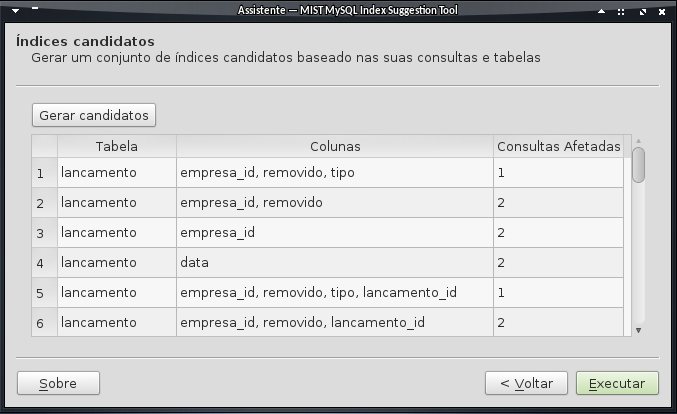
\includegraphics[width=\textwidth]{mist-indices-candidatos.png}
  \fonte{Elaborado pelo autor.}
  \label{fig:mist-candidatos-gerados}
\end{figure}

\section{Verificação dos índices candidatos}
\label{verificacao-custo-indices-candidatos}

A etapa de verificação dos índices candidatos consiste em analisar o custo de execução de todas as consultas avaliadas utilizando cada índice candidato que pode afetar a sua performance. Esta análise de custo é realizada utilizando-se o comando EXPLAIN do MySQL em um banco de dados com todas as tabelas e índices candidatos criados.

O banco de dados utilizado para o processo de verificação dos índices deve ser uma cópia do banco de dados original, com todas as tabelas e dados armazenados. Apenas os índices secundários já existentes devem ser removidos, de forma a não afetar os resultados do otimizador do MySQL durante as execuções das consultas.

Cada índice candidato gerado na etapa anterior é criado no banco de dados individualmente e todas as consultas que são afetadas por ele são avaliadas. Em seguida, o índice é removido do banco de dados e o próximo candidato é avaliado. Este processo se repete até que todos os índices candidatos tenham sido avaliados, conforme ilustrado na figura \ref{fig:verificacao-custo-candidatos}.

\begin{figure}[!hbt]
  \centering
  \caption{Processo de verificação dos índices candidatos.}
  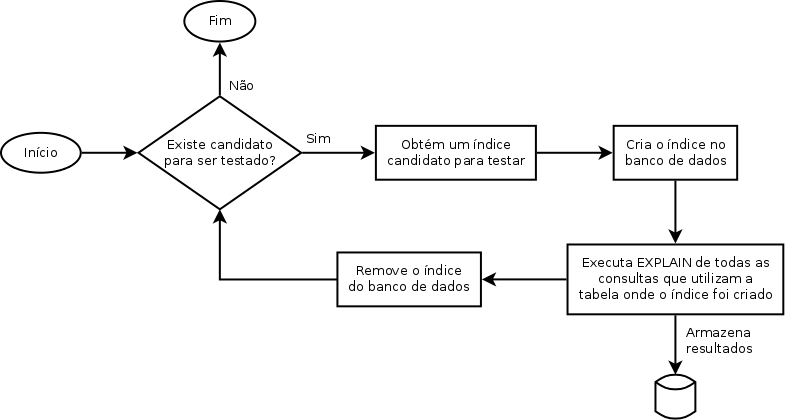
\includegraphics[width=\textwidth]{verificacao-custo-candidatos.png}
  \fonte{Elaborado pelo autor.}
  \label{fig:verificacao-custo-candidatos}
\end{figure}

A avaliação das consultas é realizada através de instruções EXPLAIN, que são enviadas para o servidor do banco de dados MySQL. Para ser possível obter as informações necessárias para o MIST, deve ser utilizada a versão 5.7 ou superior do servidor MySQL. O valor do custo da consulta é retornado pelo servidor MySQL no formato \gls{json}, e é salvo pelo MIST vinculado ao índice utilizado e à consulta verificada. Este valor é utilizado posteriormente para gerar a solução final, como descrito na seção \ref{geracao-solucao-final}.

\section{Geração de solução final}
\label{geracao-solucao-final}

Após executar as etapas de verificação de custo para todos os índices candidatos gerados, a solução final é formada escolhendo-se os índices que apresentaram o menor custo para a execução das consultas, ao mesmo tempo em que podem ser aproveitados pela maior quantidade de consultas diferentes. Um fluxograma de como esse processo é realizado é apresentado na figura \ref{fig:escolha-solucao-final}.


\begin{figure}[!htb]
  \centering
  \caption{Fluxograma para escolha dos índices da solução final.}
  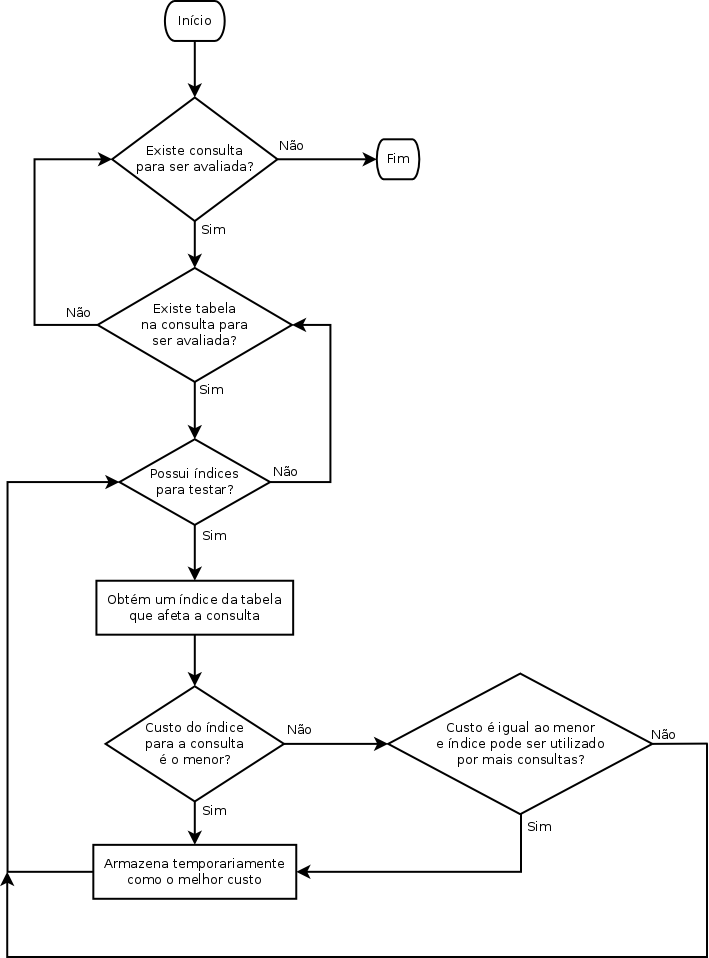
\includegraphics[width=\textwidth]{escolha-solucao-final.png}
  \fonte{Elaborado pelo autor.}
  \label{fig:escolha-solucao-final}
\end{figure}


O algoritmo de escolha dos índices para a solução final percorre todas as consultas que foram analisadas e, para cada tabela utilizada na consulta, escolhe o índice candidato com o menor custo. Em caso de dois ou mais índices oferecerem o mesmo custo, a ferramenta irá optar pelo índice que possa ser utilizado por mais consultas, eliminando a necessidade de índices adicionais e evitando que sejam escolhidos índices muito específicos.



\chapter{Conclusão}
\label{conclusao}

A otimização da performance de bancos de dados é de vital importância para a vasta maioria dos sistemas existentes no mercado que utilizado o modelo de dados relacional. Dado o rápido crescimento da quantidade de dados a ser armazenada por estes sistemas, o desempenho destes deve ser aprimorado continuamente.

Para atingir o objetivo proposto neste trabalho, foi desenvolvida uma ferramenta capaz de recomendar opções de índices para serem utilizados em um banco de dados analisado, visando reduzir o custo de processamento das consultas no servidor.

Na tabela \ref{tab:trabalhos-relacionados}, apresentada no capítulo \ref{trabalhos-relacionados}, foram listados alguns dos trabalhos já desenvolvidos por outros autores da área e foi realizada uma comparação entre as contribuições dos mesmos. Retornando-se a esta tabela, pode-se agora incluir as características da aplicação desenvolvida (tabela \ref{tab:contribuicao-trabalho}).

\begin{table}[H]
  \centering
  \caption{Contribuição do trabalho desenvolvido}
  \begin{tabular}{|p{2.1cm}|l|p{3.4cm}|p{2.1cm}|p{4.1cm}|} \hline
    \textbf{Trabalho}
        & \textbf{SGBD}
        & \textbf{Objetivo}
        & \textbf{Abordagem}
        & \textbf{Avaliação de custo}
        \\ \hline

    Weiland e Kroth, 2016
        & MySQL
        & Sugestão de índices
        & \emph{Offline}
        & Consultas ao otimizador do \gls{sgbd} utilizando índices materializados
        \\ \hline
  \end{tabular}
  \label{tab:contribuicao-trabalho}
  \fonte{Elaborado pelo autor.}
\end{table}

Os resultados obtidos com a ferramenta desenvolvida neste trabalho foram satisfatórios. Porém, pode-se observar ainda que existem vários ajustes que poderiam ser desenvolvidos na busca de melhores resultados. Em comparação aos trabalhos relacionados, o MIST ainda não possui algumas funcionalidades que seriam muito úteis, porém que não foram implementadas devido ao escopo e tempo limitado do trabalho.

A primeira melhoria detectada refere-se à entradas dos dados na ferramenta. A solução desenvolvida, utilizando arquivos \gls{xml}, ainda exige um processamento manual dos dados para formatá-los de acordo com o esperado pela ferramenta. Idealmente, o MIST poderia conectar-se diretamente a um banco de dados configurado para obter todas as informações essenciais sobre as tabelas e estatísticas sobre os dados, sem a necessidade de intervenção manual.

Também referente à entrada de dados, o MIST poderia ser integrado com o \emph{parser} do MySQL de modo a interpretar as consultas a serem analisadas sem exigir uma conversão manual destas para um arquivo \gls{xml}. Além disso, esta integração possibilitaria que o MIST avaliasse consultas mais complexas, incluindo união e sub-consultas. Adicionar suporte para avaliar instruções de atualização de dados, como INSERTs e UPDATEs, também seria uma funcionalidade importante para a ferramenta.

Outras melhorias identificadas são relacionadas à otimização do programa, que pode ser obtida de duas formas: 1) utilização de melhores heurísticas para a geração de índices candidatos, de forma a gerar uma quantidade menor de índices para serem verificados no banco de dados; ou 2) implementação do suporte a simulação de índices no MySQL, removendo a necessidade da criação dos índices materializados e utilizando apenas as estatísticas calculadas sobre os dados.


\bibliography{referencias}

% Anexos

\end{document}
